\section{Implementierung}

\subsection{Klassendiagramm}
\begin{minipage}[b]{0.5\linewidth}
\centering
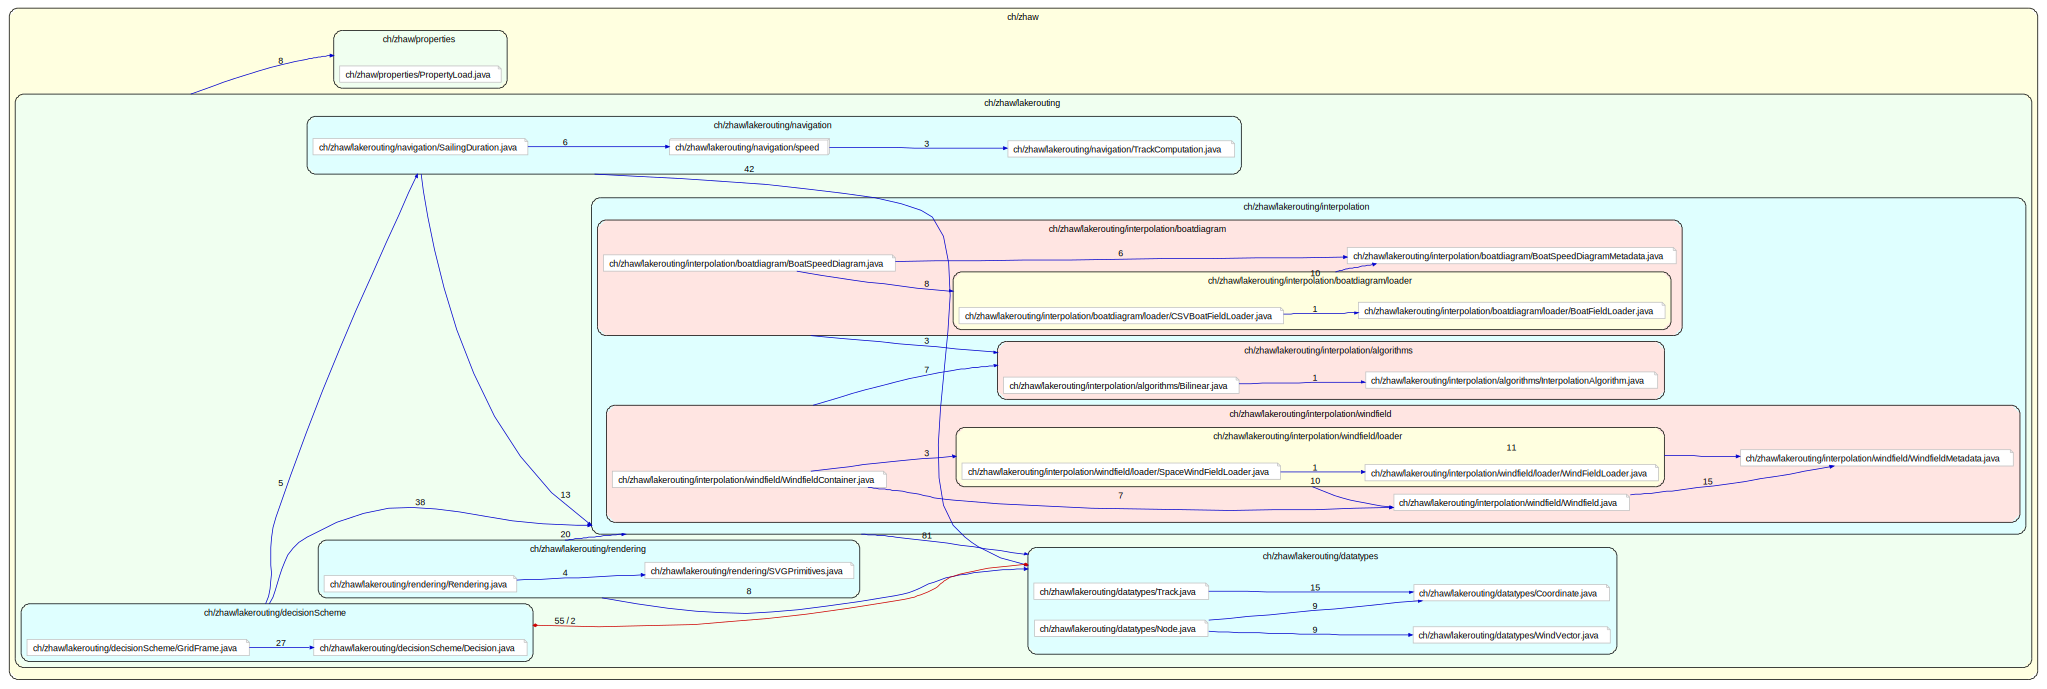
\includegraphics[width=\textheight, angle=90]{img/ArchInternalDependencies-ch}
\end{minipage}
\hspace{0.5cm}
\begin{minipage}[b]{0.5\linewidth}
\centering
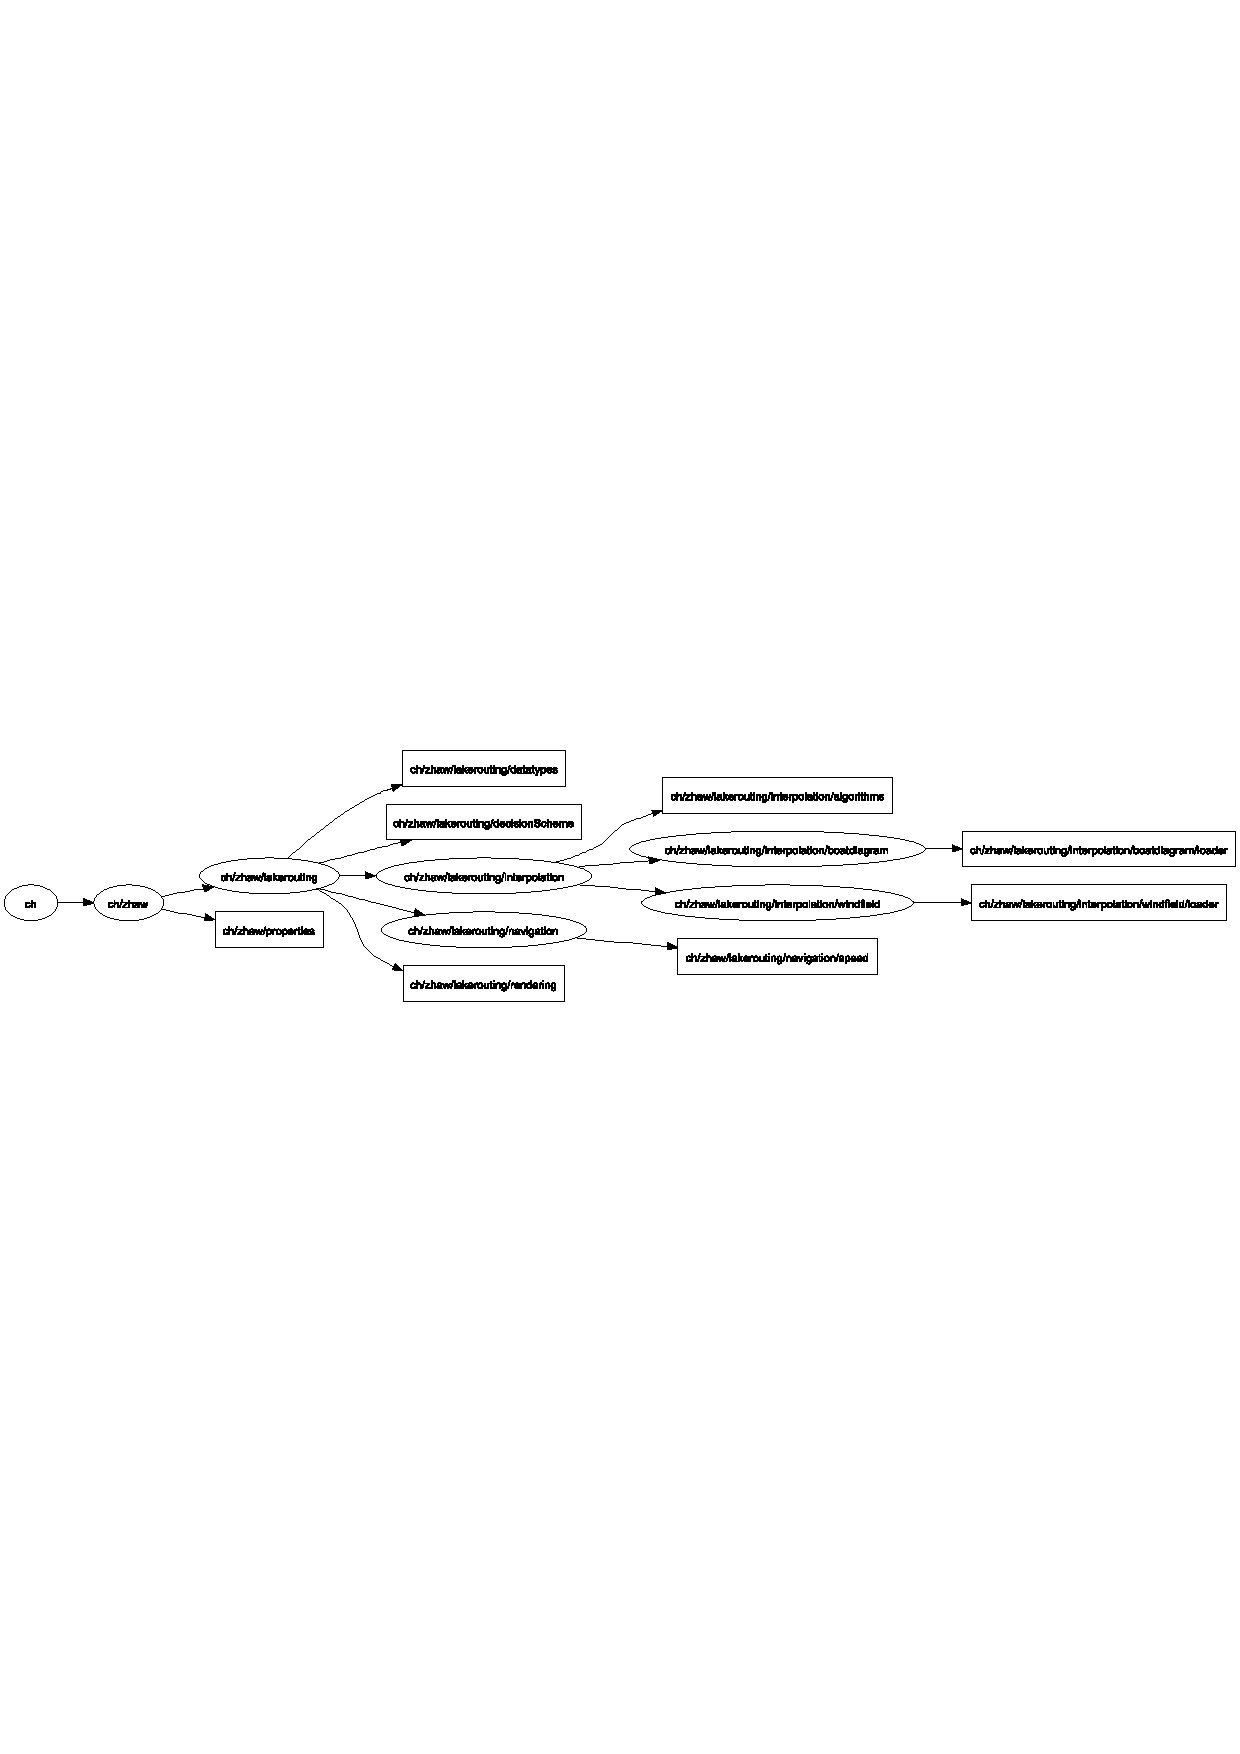
\includegraphics[width=\textheight, angle=90]{img/ArchitectureGraph-ch}
\end{minipage}


\subsection{Decision}
Die Klasse $Decision$ ist die Hauptklasse unserer Applikation. Alle wichtigen Variablen wie \texttt{logger}, \texttt{graphList} oder \texttt{windfieldContainer} werden in dieser Klasse initialisiert und berechnet. Ausserdem findet die sogenannte dynamische Programmierung auch hier statt. 

Die dynamische Programmierung wurde so umgesetzt, dass es eine Methode namens \texttt{progdyn()} gibt, welche in einer \texttt{for}-Schleife merhmals aufgerufen wurde. Als Parameter wird dieser Methode die Spaltennummer und der Windfeld-index übergeben. Danach werden über alle Knoten dieser Spalten und alle Knoten der vorherigen Spalte die Berechnungen durchgeführt. Für jeden Knoten dieser Spalte werden die Verbindungen berechnet und die Ergebnisse in einem Array abgespeichert. Anschliessend wird dann die kürzeste Verbindung ermittelt und in den globalen ArrayList \texttt{graphList} eingetragen. 

\lstinputlisting[label=src:decision,caption=Aufruf der dynamischen Methode]{code/decision.java}

\subsection{GraphList}
Wie in Abschnitt \ref{aufg6:entscheidungsbaum} erklärt wurde, brauchen wir
eine Liste, die alle nötigen Informationen zu den Knoten beinhaltet. Da die
Grösse des Arrays variabel ist und wir zum grössten Teil einen index-basierten
Zugriff benötigen, haben wir uns entschieden die Datenstruktur
$java.util.ArrayList$ mit Generics zu verwenden. Eine generische ArrayList
erlaubt es genau zu definieren, welche Elemente/Datentypen einer ArrayList
hinzugefügt werden dürfen. Ausserdem brauchen wir für eine tabellarische Form
ein 2-dimensionales ArrayList. Um dies zu erreichen, wird ein ArrayList in
einem ArrayList definiert. Somit entspricht der erste ArrayList der Spalten
und die zweite der Zeilen dieser Spalten.

Dementsprechend sieht die Initialisierung des ArrayLists so aus:

\lstinputlisting[label=src:graphListInitialization,caption=Initialisierung der Liste]{code/graphlist_initialize.java}

\subsubsection{Node}
Für die Speicherung der Daten wurde eine Klasse $Node$ erstellt, welche die
Werte über die Knoten beinhaltet. Weil wir nun mehrere Informationen zu den
einzelnen Knoten haben, haben wir uns entschieden, neben den Auflistungen in
\ref{aufg6:entscheidungsbaum} auch noch weitere Daten in der Liste
abzuspeichern, um Redundanz zu vermeiden. Deshalb werden neu auch Koordinaten
zu den Knoten und die dazugehörigen Windvektoren in der Liste abgelegt.

Demzufolge enthält die Klasse folgende Informationen:

\begin{itemize}
\item \textbf{TimeOfArrival}: Die Dauer vom Anfangsknoten bis zu diesem Knoten.
\item \textbf{Previous Node}: Die Referenz zum vorherigen Knoten.
\item \textbf{Coordinate}: Breiten- und Längengrade des Knotens.
\item \textbf{WindVektor}: Der Windvektor $(u, v)$ an diesem Knoten.
\end{itemize}

Desweiteren erbt diese Klasse von der Interface $Comparable$, um Vergleiche
zwischen den Knoten zu ermöglichen. Infolgedessen ist es möglich, die Klasse
$Collections$ zu benutzen, welche nützliche Methoden für Listen wie \texttt{min()},
\texttt{max()}, \texttt{sort()} etc. enthält. Wir machen in unserem Code von der
\texttt{min()}-Methode Gebrauch, um den Knoten mit dem kleinsten TimeOfArrival in
einer Spalte zu finden.

Als nächstes wurde innerhalb der ArrayList eine sogenannte LinkedList
implementiert. Jeder Knoten beinhaltet eine Referenz zum vorherigen Knoten und
der Anfangsknoten hat eine Referenz auf sich selbst. Dementsprechend braucht
man nicht durch alle Knoten zu iterieren um einen Pfad zu zeichnen, sondern es
reicht den Knoten zu wählen, von dem man den Pfad zum Anfang zeichnen möchte.

Die Implementation der Klasse $Node$ sieht wie folgt aus:

\lstinputlisting[label=src:nodeClass,caption=Node-Class]{code/node.java}


\subsubsection{Coordinate}
Um die Koordinaten der Knoten in der Klasse $Node$ abspeichern zu können,
haben wir eine Klasse $Coordinate$ erstellt. Normalerweise werden die
GPS-Koordinaten im Format N 47\degree 12' 45" E 12\degree 45' 30" oder 47.2125
Längengrad and 12.758333 Breitengrad gebraucht. Aber es kann durchaus sinnvoll
sein, diese Angaben auch in Radian zu haben, wie bei der Berechnung der
Orthodromie es der Fall ist. 

Damit wir nicht zwei Datentypen für diese zwei Einheiten erstellen müssen,
werden diese jeweils mit einem Getter \& Setter jeweils gesetzt und erhalten.
Da wir nicht vier Variablen erstellen möchten, zwei für Grad und zwei für
Radian, und die Klasse an sich selbst auch nichts über den Inhalt wissen muss,
ist es von Vorteil, die zwei Einheiten nur nach Aussen zu unterscheiden und im
internen als eine einzige Einheit zu behandeln. Das bedeutet, dass die Werte
intern nur in Grad gehandhabt werden und bei Bedarf nach Aussen in Radian
umgerechnet werden. Es ist aber auch möglich die GPS-Koordinaten in Radian zu
setzen, welches im internen in Grad umgerechnet und abgespeichert wird. 

Somit kann diese Klasse jederzeit erweitert und neue "Formate" hinzugefügt
werden, ohne die Funktionalität zu beeinträchtigen.

Die Implementation der Klasse $Coordinate$ sieht wie folgt aus:

\lstinputlisting[label=src:crdClass,caption=Coordinate-Class]{code/coordinate.java}

\subsubsection{Windvector}
Ein Windvektor ist nichts anderes als ein Komposit von zwei normalen Vektoren und
beinhaltet weitere zwei Getter-Methoden für die häufig verwendeten Berechnunungen 
wie die Windgeschwindigkeit und die Winkel. Der Vektor $u$ zeigt in den Norden 
und der Vektor $v$ zeigt in den Osten. Aus diesem Grund wird die Geschwindigkeit 
durch den Betrag der zwei Vektoren berechnet. Und der Winkel lässt sich mit dem 
Arkuskosinus von Vektor $u$ und der Windgeschwindigkeit berechnen, wobei der
Winkel von Norden im Uhrzeigersinn zeigt.

\lstinputlisting[label=src:windvectorClass,caption=WindVector-Class]{code/windvector.java}


\subsection{Polar-Diagramm}
\subsubsection{Parser}

Die Schiffsdaten sind als CSV\footnote{Comma Separated Values}-Datei gegeben
und werden von einem selbst\-geschriebenen Parser in ein passendes
Klassen-Konstrukt geladen. Die Schwierigkeit bestand darin, dass die Daten
nicht-dekoriert sind und daher nur durch ihre Position von anderen Typen zu
unterscheiden sind. Das bedeutet allerdings auch, dass der Parser sich auf
diese Datenstruktur verlässt und keine Abweichungen duldet und sonst abstürzt.

Dieses Problem ist allerdings vertretbar, da die Datenstruktur vorgegeben ist
und der Parser daran angepasst wurde. Es ist im Allgemeinen sehr schwierig
einen Parser für eine schwach typisierte Datenstruktur zu schreiben. Eine
robustere Datenstruktur würde XML bieten, die strikte Einschränkung bis hin zu
Datentypen für einzelne Felder bietet.

\subsubsection{Verarbeitungsklasse}
Die Klasse \texttt{BoatSpeedDiagram.java\footnote{Im Package
ch.zhaw.lakerouting.interpolation.boatdiagram zu finden}} verwaltet das
Polardiagram und bietet die nötigen Methoden für die Abfrage der Werte an,
kapselt die Interpolation, so das der Programmierer sich darum nicht kümmern
muss.

\subsubsection{Bilineare Interpolation}\label{sss:bilinearinterpolation}
Die Interpolation an sich ist durch 
\begin{equation}
f(x,y) \approx \begin{bmatrix} 1-x & x \end{bmatrix} \begin{bmatrix}
f(0,0) & f(0,1) \\ f(1,0) & f(1,1) \end{bmatrix} \begin{bmatrix} 1 - y
\\ y \end{bmatrix}
\label{eq:bilineareinterpolation}
\end{equation}
geben und kann in Java wie nachfolgend gezeigt, implementiert werden.

 \lstinputlisting[label=src:bilinearinterpolation,caption=Bilineare Interpolation]{code/BilinearInterpolation.java}
Die konkrete Berechnung erfolgt auf den Zeilen 17-19 und zeigen den einfachen
Charakter der Berechnung. Diese Implementation erfordert allerdings eine
geringe Aufbereitung der Eingabewerte, ist dafür einfacher zu testen und somit
indirekt auch weniger anfällig für Implementationsfehler, was direkt zu
robusterem Code führt.

\subsection{Windfelder}
Die Implementation ist vergleichsweise einfach gehalten und besteht aus einer
Klasse für ein einzelnes Windfeld mit Hilfsfunktionalitäten für die
Interpolation der Windvektoren und das Abfragen der Nachbarsvektoren an einer
bestimmten Position. Diese einzelnen Windfelder werden dann in einem Art Stapel
aufbewahrt\footnote{Wir verwenden der Einfachheit halber ein normales Array.}
Im Prinzip besteht das alles aus einer dreidimensionalen Struktur aus
Windvektoren.

\subsubsection{Windfeld-Parser}
Der Parser ist ein Eigenbau und wurde speziell für diese Datenstruktur
geschaffen. Diverse Unzulänglichkeiten wie nicht-leere Zeilen und Trailing
Spaces haben die Entwicklung erschwert und dementsprechend viel Zeit gekostet.

Allerdings lässt sich der Parser leicht auf andere Ressourcen erweitern wie zum
Beispiel HTTP und erlaubt auch die direkte Anbindung an Datenbanken.

Das Prinzip vom Parser ist einfach: Er öffnet die Datei, versucht den Header
des Windfeldes zu erkennen, liest diesen ein. Alle nachfolgenden Zeilen des
Blocks werden als Windfeld-Daten interpretiert. Erscheint eine Leerzeile wird
der Block als abgeschlossen betrachtet und er versucht den nächsten Header zu
erkennen. Grafisch sieht der Controllflow wiefolgt aus:

\begin{center}
 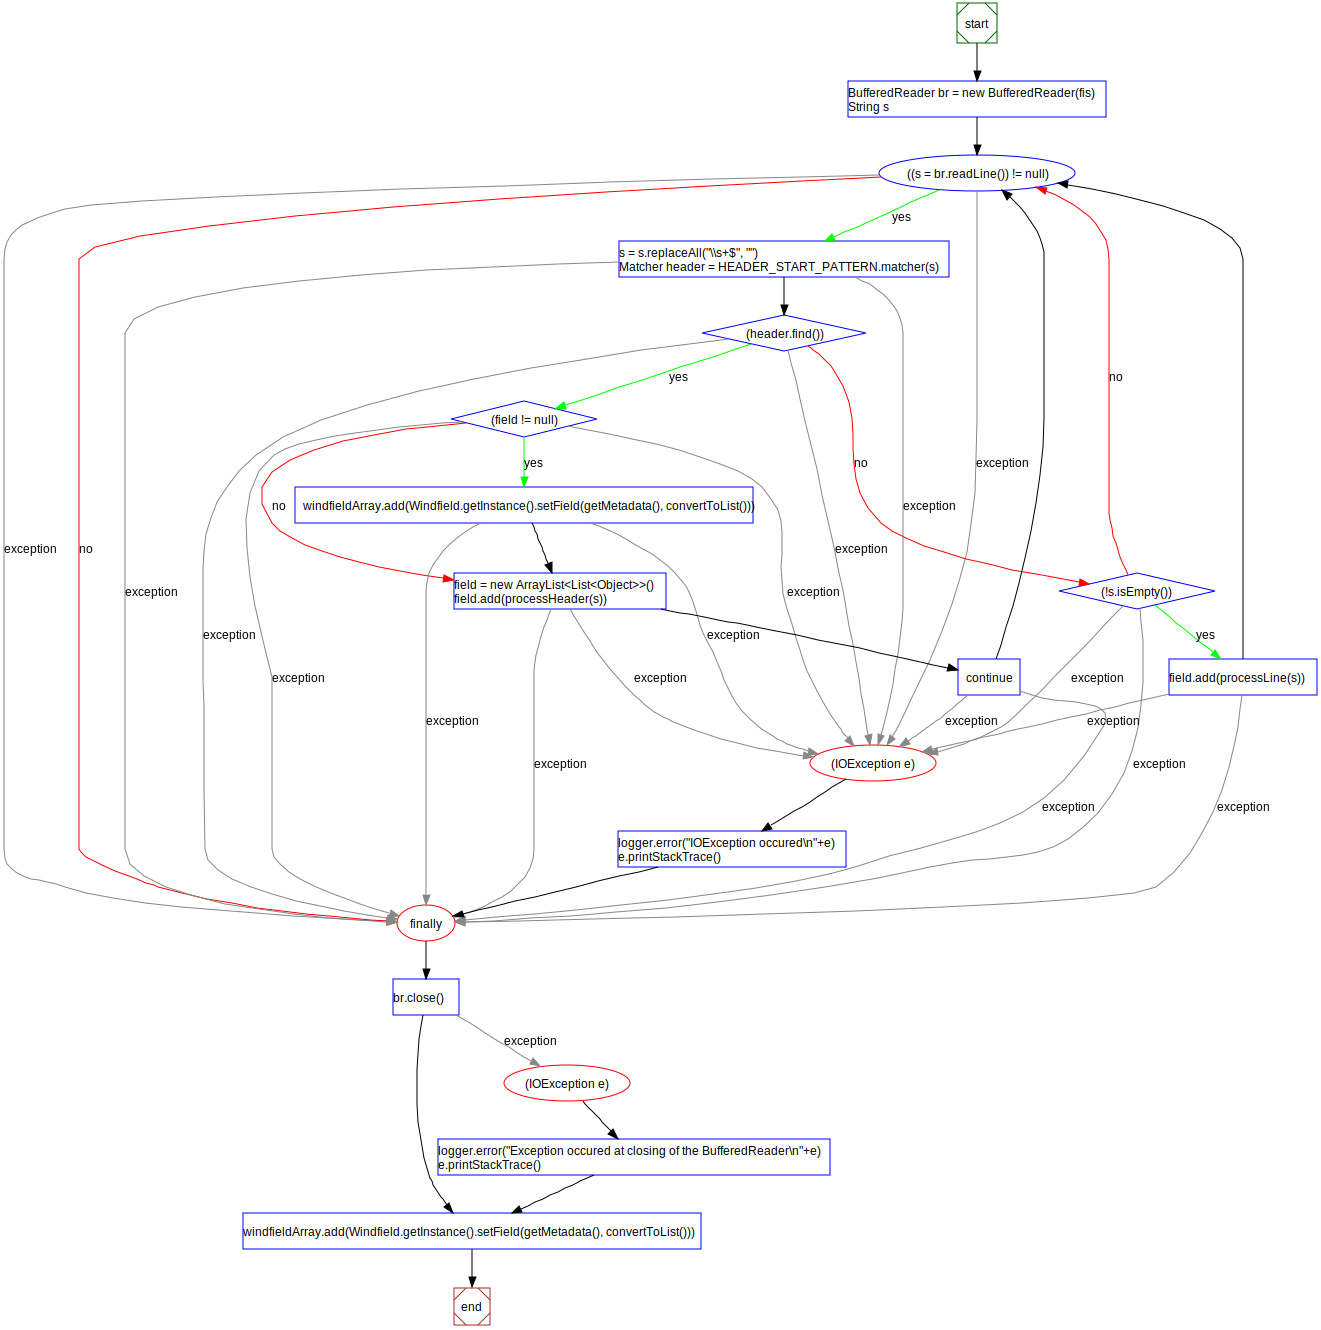
\includegraphics[width=0.8\linewidth]{img/ControlFlowGraph-SpaceWindFieldLoader-read}
\end{center}

\lstinputlisting[label=src:windfieldparser,caption={Windfield-Parser,
Codeausschnitt der relevanten Funktionen}]{code/spacewindfieldloader.java}

\subsubsection{Interpolation der Windvektoren}
Da das Windfeld und das Entscheidungsnetz nicht über dieselben Koordinaten
verfügen und dementsprechend die Entscheidungspunkte normalerweise zwischen den
Windvektoren zu liegen kommen, wird nach Berechnung des Entscheidungsnetzes dem
Windfeld die Koordinatenliste übergeben. Das Windfeld interpoliert die
Windrichtung bzw. die Windvektoren an den geforderten Positionen. Das erfolgt
wie bereits in Abschnitt \ref{sss:bilinearinterpolation} erklärt über dieselbe
Klasse.

Nach dieser initialen Interpolation verfügen das Entscheidungsnetz und das
Windfeld über dieselben Array-Indizes und können somit leicht (wieder-)
verwendet werden.

\subsection{Properties}
Ein weiteres Problem stellten die verschiedenen Systemen dar, auf welchen diese Applikation laufen gelassen wurde. Die Pfade der Dateien, die in der Applikation eingelesen werden, stimmten nicht überein und bei jeder Übernahme der Änderungen mussten die Pfade angepasst werden. Desweiteren sind statische Pfade im Code unerwünscht, da sie später dem Entwickler viel Probleme bereiten können. 

Aus diesem Grund haben wir uns entschieden, eine Properties-Datei zu erstellen, welche als einfacher Konfigurationsmechanismus verwendet wird. In dieser Datei werden Variablen Werte zugewiesen, welche dann im Programm benutzt werden können. 

Nachfolgend wie die Konfigurations-Datei aussieht:
\lstinputlisting[label=src:configurationProp,caption=Konfigurations-Datei]{code/configuration.properties}

Eine solche Properties-Datei kann mittels der Klasse $java.util.Properties$ eingelesen werden. Dafür haben wir eine eigene Klasse $PropertyLoad$ geschrieben, um uns Tipparbeit zu ersparen und die Handhabung der ganzen Einlesen/Auslesen zu erleichtern. Dieser Klasse wird der Name der Variablen übergeben und es liefert als Ergebnis den Wert zurück, welcher in der Properties-File zu finden ist.

Die Implementierung der Klasse $PropertyLoad$:
\lstinputlisting[label=src:propLoad,caption=PropertyLoad-Klasse]{code/propertyLoad.java}

\subsection{Logging}
% TODO: Quellen angeben
Für das Logging wird die Log4j-Library von Apache Software Foundation verwendet. Dieses Framework
erlaubt uns, mehrere Loggingsysteme zu defnieren und die Standardausgaben über sogenannte Logger an sie
weiterzuleiten. Somit ist es zum Beispiel möglich, die Meldungen gleichzeitig in einer Datei, an einem Syslog-
Daemon und auf der Konsole auszugeben. Die Library ermöglicht sehr flexible Konfigurationen. Die Abhängigkeiten sind gering, man muss nur eine JAR-Datei als Library in das Projekt hinzufügen, gleiches gilt für die Verwendung: Eine einfache Verwendung ohne grosse Einarbeitungszeit ist hier möglich.

Wir haben uns für den Logging entschieden, da die Konsolenausgaben viel Performance beanspruchen und diese Ausgaben nach der Schliessung der Anwendung verschwinden. Diese Ausgaben können zum Teil sehr behilflich sein, wie z.B. die Fehlerquelle zu identifizieren oder herauszufinden, was als letztes ausgeführt wurde. 

Deswegen werden jetzt die Ausgaben in eine Datei namens $lakeRouting.log$ umgelenkt. Falls die Grösse der Datei die maximale Grösse von 10MB erreicht, wird diese Datei mit dem Datum versehen und eine neue Datei mit dem gleichen Namen angelegt. 

Dies wurde erreicht, indem man mit der unten aufgeführten log4j.properties-Datei die Konfiguration einliest. Das Einlesen der Properties-Datei erfolgt nur an einer einzigen Stelle im ganzen Projekt, da es nur einmal geladen werden muss und die Einstellungen dann für die ganze Runtime\footnote{Zeitspanne, während der ein Programm von einem Rechner ausgeführt wird} gültig sind.

\lstinputlisting[label=src:log4jProperties,caption=Properties-Datei der Log4j]{code/log4j.properties}
